\documentclass[conference]{IEEEtran}
\IEEEoverridecommandlockouts
% The preceding line is only needed to identify funding in the first footnote. If that is unneeded, please comment it out.
\usepackage{cite}
\usepackage{amsmath,amssymb,amsfonts}
\usepackage{algorithmic}
\usepackage{graphicx}
\usepackage{textcomp}
\usepackage{xcolor}
\usepackage{booktabs}
\usepackage{subcaption}
\usepackage{multirow}
\usepackage{svg}
\usepackage{hyperref}

\DeclareMathOperator*{\argmax}{arg\,max}
\def\eg{\emph{e.g. }}
\def\Eg{\emph{E.g.}}
\def\etal{\emph{et al. }}
\def\ie{\emph{i.e. }}
\def\Ie{\emph{I.e. }}


\def\BibTeX{{\rm B\kern-.05em{\sc i\kern-.025em b}\kern-.08em
    T\kern-.1667em\lower.7ex\hbox{E}\kern-.125emX}}
\begin{document}

\title{Towards Clear Evaluation of Robotic Visual Semantic Navigation \\
\thanks{This research was funded by projects: AIRPLANE, with reference PID2019-104323RB-C31; EYEOT, with reference PID2021-128362OB-100; and POLLUTWIN, with reference TED2021-129162B-C22 from the Ministry of Science and Innovation of Spain.}
}

% \author{\IEEEauthorblockN{1\textsuperscript{st} Given Name Surname}
% \IEEEauthorblockA{\textit{dept. name of organization (of Aff.)} \\
% \textit{name of organization (of Aff.)}\\
% City, Country \\
% email address}
% \and
% \IEEEauthorblockN{2\textsuperscript{nd} Given Name Surname}
% \IEEEauthorblockA{\textit{dept. name of organization (of Aff.)} \\
% \textit{name of organization (of Aff.)}\\
% City, Country \\
% email address}
% \and
% \IEEEauthorblockN{3\textsuperscript{rd} Given Name Surname}
% \IEEEauthorblockA{\textit{dept. name of organization (of Aff.)} \\
% \textit{name of organization (of Aff.)}\\
% City, Country \\
% email address}
% }

\author{
\IEEEauthorblockN{
Carlos Guti\' errez-\'Alvarez\IEEEauthorrefmark{1}, Sergio Hern\'andez-Garc\'ia\IEEEauthorrefmark{2}, Nadia Nasri\IEEEauthorrefmark{1}\IEEEauthorrefmark{3}, \\ Alfredo Cuesta-Infante\IEEEauthorrefmark{2} and Roberto J. L\'opez-Sastre\IEEEauthorrefmark{1}}
\IEEEauthorblockA{\IEEEauthorrefmark{1}University of Alcal\'a, Department of Signal Theory and Communications, Alcal\'a de Henares, Spain\\
Email: \{carlos.gutierrezalva, nadia.nasri, robertoj.lopez\}@uah.es}
 \IEEEauthorblockA{\IEEEauthorrefmark{2}Rey Juan Carlos University, Superior Polytechnic School of Computer Science, M\'ostoles, Spain\\
Email: \{sergio.hernandez, alfredo.cuesta\}@urjc.es}
\IEEEauthorblockA{\IEEEauthorrefmark{3}University of Alicante, Institute for Computer Research, Alicante, Spain}
}


\maketitle

\begin{abstract}
In this paper we address the problem of visual semantic navigation (VSN), in which a robot needs to navigate through an environment to reach an object having only access to egocentric RGB perception sensors.
This is a recently explored problem, where most of the approaches leverage last advances in deep learning models for visual perception, combined with reinforcement learning (RL) strategies.
Nonetheless, after a review of the literature, it is complicated to perform direct comparisons between the different solutions.
The main difficulties lie in the fact that the navigation environments in which the experimental metrics are reported are not accessible, and each approach uses different RL libraries.
In this paper, we release a publicly available experimental setup for the VSN problem, with the aim of providing a clear benchmark.
It has been constructed using pyRIL, an open source python library for RL, and two navigation environments: Miniwolrd-Maze from gym-miniworld, and one 3D scene from HM3D dataset using AI Habitat simulator.
We finally propose a state-of-the-art VSN model, consisting in a Contrastive Language Image Pretraining (CLIP) visual encoder plus a set of two recurrent neural networks for producing the discrete navigation actions.
This model is evaluated in the proposed experimental setup, with a careful analysis of the main VSN challenges, namely: the sparse rewards problem; and the exploitation-exploration trade-off.
Code is available at: \url{https://github.com/gramuah/vsn}.
\end{abstract}

\begin{IEEEkeywords}
navigation, reinforcement learning, robot, deep learning
\end{IEEEkeywords}

\usepackage{acronym}\chapter{Introduction}\label{ch:introduction}

\setlength\epigraphwidth{.69\textwidth}
\epigraph{\itshape ---The most important step a man can take.
It's not the first one, is it?
---It's the next one.
Always the next step, Dalinar.}{Brandon Sanderson, \textit{Oathbringer.}}

\lettrine{\textcolor{accent_color}{W}}{ho} has never dreamt of a robot friend?
A robot that can help you with your daily tasks, play games with you, help you with your homework, or even be your personal assistant?
The idea of having a robotic companion is not new, for it has remained a dream for humanity for a long time.
Since the first mention of the term \textit{robot}~\cite{robot1920}, this aspiration has been only possible in science fiction movies and books.
However, with the recent advancements in robotics and \acrfull{ai}, humanity is closer than ever to this reality.
This humble thesis is nothing more than just a small step towards the joint effort of achieving this dream.

Now, how do we create a robot that can be a friend to humans?
This simple question omits a multitude of challenges that need to be addressed.
Some of these challenges include the robot's ability to understand and interact with humans, its ability to learn from its environment, or its ability to adapt to different situations.
However, there is one aspect underlying all these challenges; \textit{movement}:

\begin{itemize}
    \item A robot that understands and interacts with humans \textit{must be able to move} in order to follow the humans and interact with them.
    \item A robot that learns from its environment \textit{must be able to move} in order to explore and gather information.
    \item A robot that adapts to different situations \textit{must be able to move} in order to change its behavior and actions based on the environment.
\end{itemize}

Moreover, it has been thoroughly discussed in the literature that movement is a fundamental aspect of intelligence~\cite{Darwin1871, Arbib2005, Leisman2016, Wolpert2011, Llinas2001}.
This clearly shows that movement is a crucial component of any intelligent system known to us.
If we want to create any intelligent entity that somehow resembles our own intelligence, we must first address the problem of movement.

This thesis is dedicated to the study of movement in robots, specifically in the context of embodied \acrshort{ai}.
This topic is known as \acrfull{vsn}, in which an agent must navigate in an environment to accomplish certain tasks while only relying on visual information.
On \acrshort{vsn} there is no prior knowledge of the environment or any map that the agent can consult.
The agent must learn to navigate in the environment by exploring it and learning from its own experiences.
It has to understand the scene not only geometrically, but also semantically.
If not, it will not be able to understand the meaning of the objects in the scene and how they relate to each other.
For example, if the agent is placed in a bedroom and asked to find a fridge, it must understand that the fridge is not (typically) in the bedroom and that it must navigate to the kitchen to find it.

\acrshort{vsn} tasks are very challenging, and as one may expect, they typically need a careful design of a complex system that combines multiple components in charge of different aspects of the navigation.
Many works~\cite{newcombe2011, thrun2001, jones2011, sattler2018, Kazerouni2022, campos2021, labbe2022, zhang2018, rosinol2020, jin2023} follow this approach, and they typically rely on a combination of visual perception, semantic understanding, and navigation planning.
However, \acrshort{vsn} can be also formulated as a \acrfull{rl}~\cite{sutton2018} problem.
\acrshort{rl} is a whole artificial intelligent framework that allows an agent to learn how to act in an environment by receiving rewards for its actions.
The rewards are typically defined in terms of the agent's performance in the task, such as reaching a goal or avoiding obstacles.
By following an iterative process within the environment, the agent can learn how to maximize its rewards and complete its tasks.

The main goal of this thesis is to study the \acrshort{rl} and \acrshort{vsn} powerful combination that allows agents to be trained to navigate in an environment.
After intensive training, agents can learn to navigate by trial and error, obtaining rewards that guide them to the goal.
In figure~\ref{fig:abstract_thesis}, an abstract representation of the thesis's framework is shown.
In it, an agent, by interacting with the environment, learns to navigate to a goal.
In the environment, even though there is not a map present, the agent can learn to understand the scene and the objects in it.
By these semantic cues, the agent can learn to navigate to the goal, even if it is not visible in the scene.

\begin{figure}
    \centering
    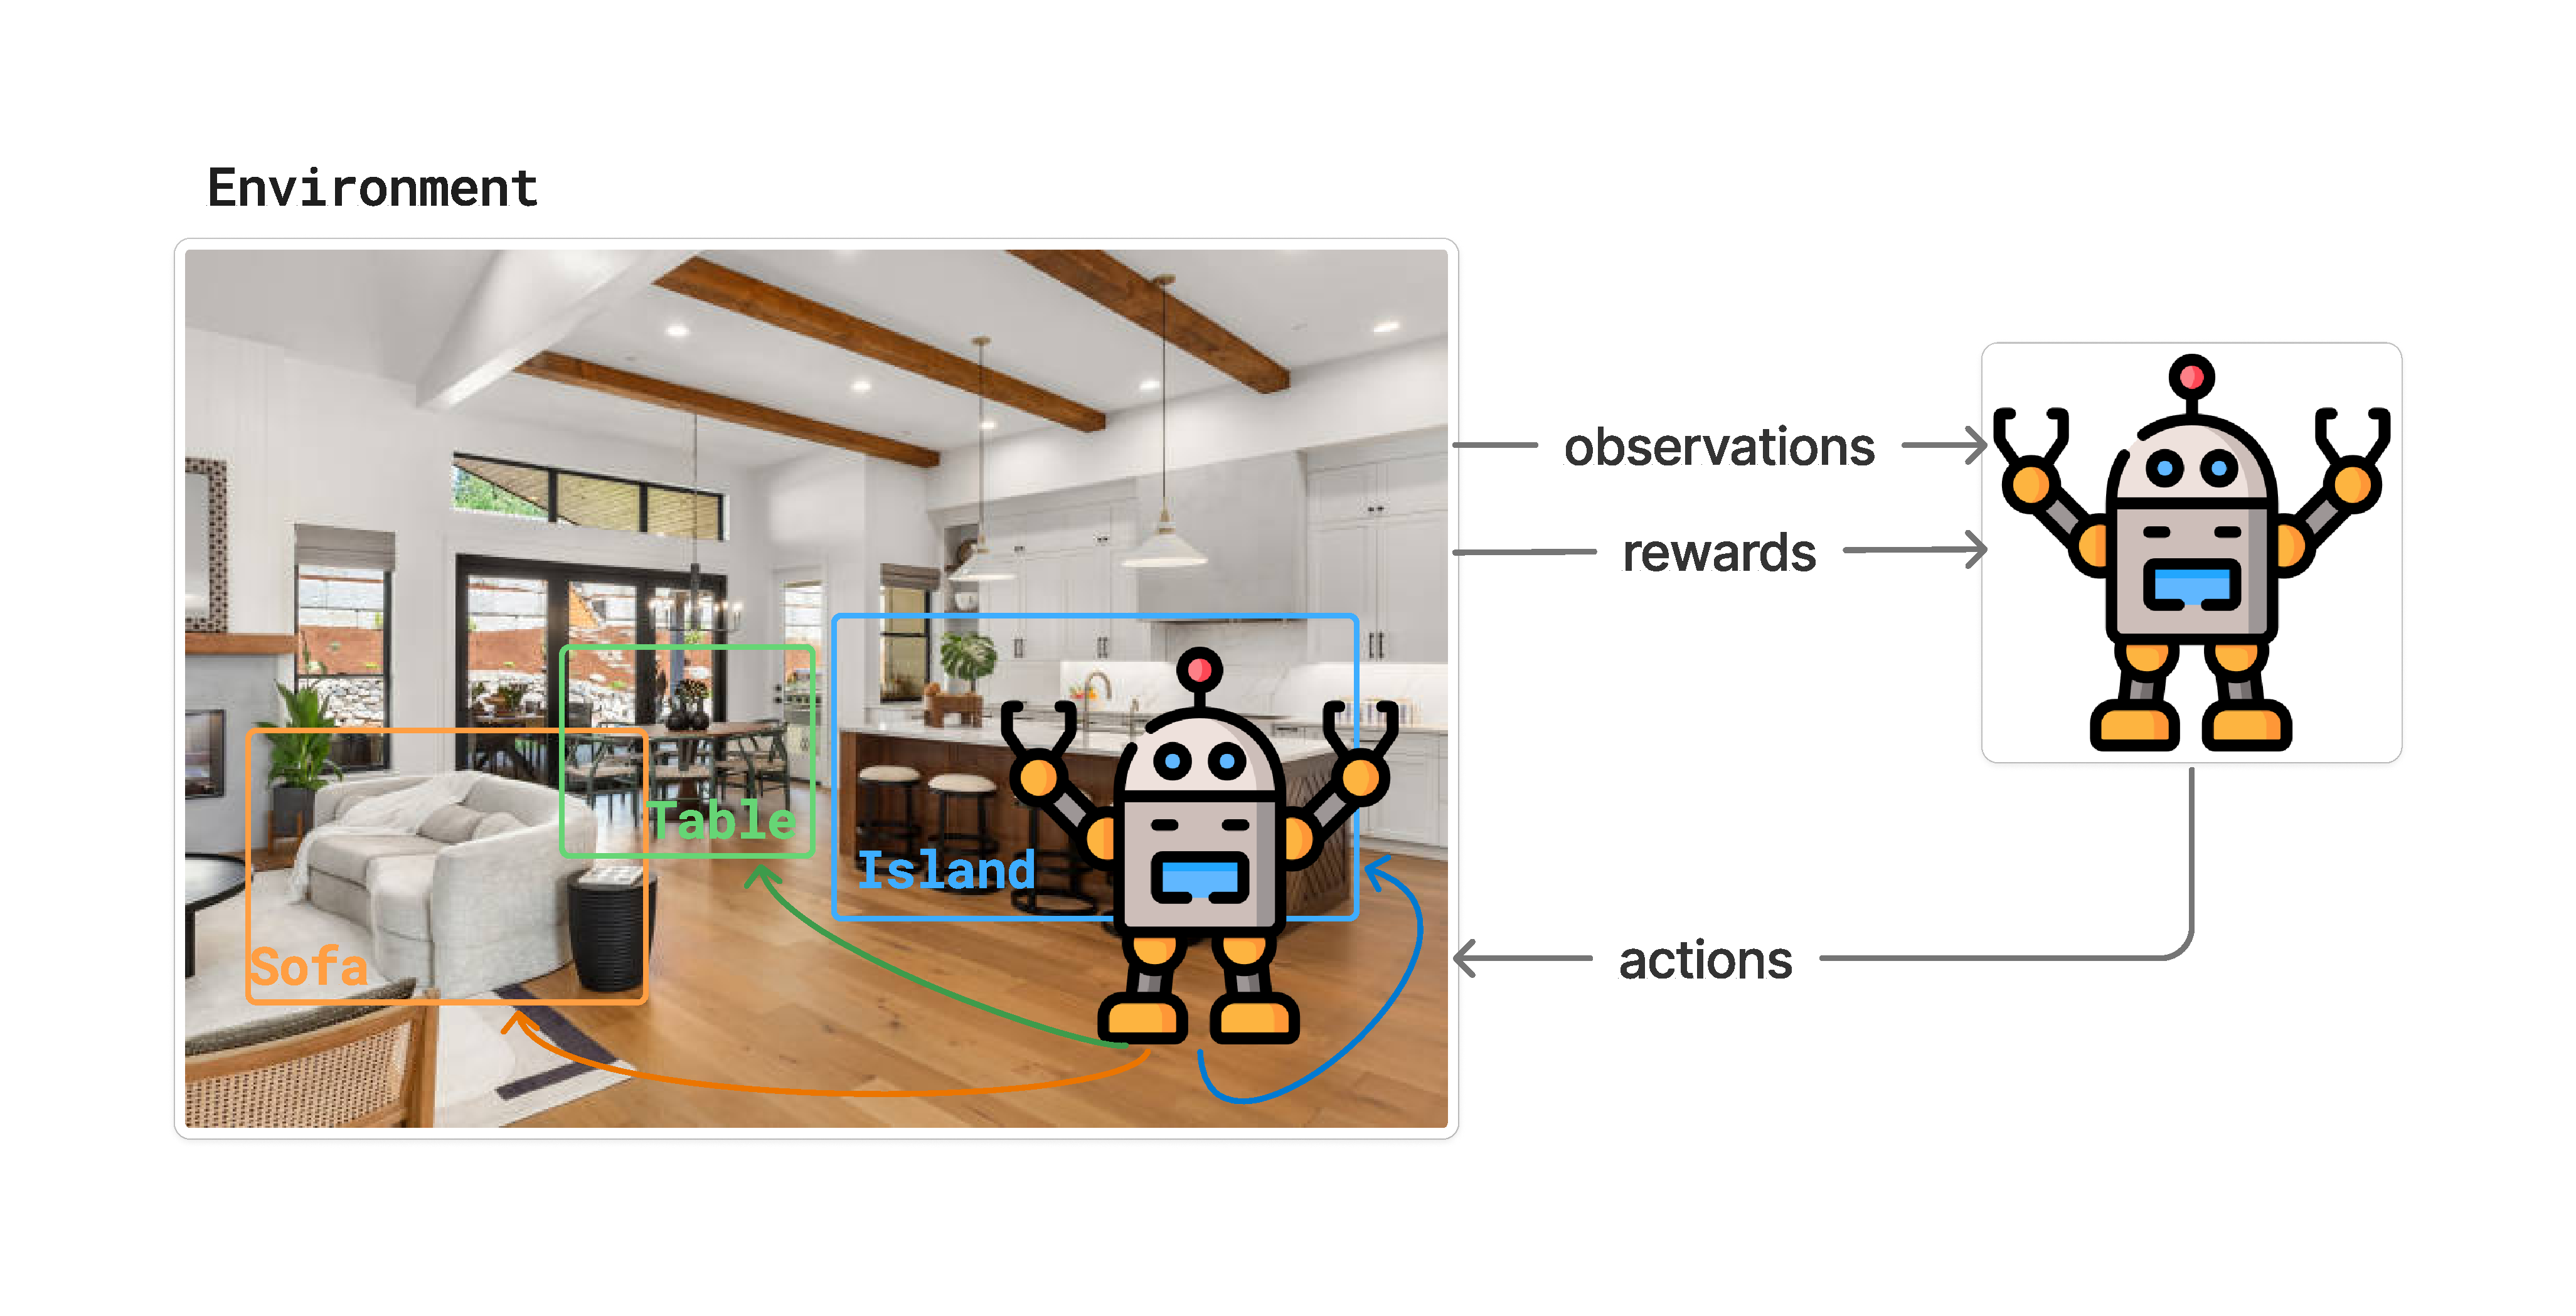
\includegraphics[trim=30 30 30 30, clip, width=\textwidth]{figures/introduction/abstract_thesis}
    \caption{\textbf{The framework of \acrshort{rl} and \acrshort{vsn}}.
    Navigating in an environment is a complex task that requires the agent to learn how to interact with the environment and understand the scene.
    The agent learns to navigate by trial and error, obtaining rewards that guide it to the goal. In this way, the agent can learn to understand the scene and the objects in it, even if there is no prior knowledge of the environment or any map that it can consult.}
    \label{fig:abstract_thesis}
\end{figure}

\section{Motivation}\label{sec:motivation}

This thesis is part of the AIRPLANE (\acrfull{ai} and Robotic Mobile PLAtforms to Improve Disabled People INdependencE) research project conducted in the~\href{https://gramweb.uah.es/}{GRAM research group} of the~\href{https://www.uah.es/en/}{University of Alcalá}.
The AIRPLANE project focuses primarily on creating new mobile robotic platforms that incorporate advanced perception, interaction, and navigation capabilities to enhance the independence of people with functional diversity.
The main goal in the AIRPLANE project is to build a low-cost mobile platform that integrates the latest advances in \acrshort{ai} and computer vision.
Specifically, it will equip the platform with the ability to navigate real environments and develop online action-recognition solutions that enable interaction applications for users with functional diversity.
And, as shown in the figure~\ref{fig:icra_papers}, the interest in this topic is not only limited to the AIRPLANE project, but it is also a hot topic in the robotics community.
Therefore, the first step is to study \acrshort{vsn} solutions that allow the robot to navigate using \acrshort{rl} algorithms.

The \acrshort{vsn} problem is very broad, and it can be applied to many different scenarios.
For example, it can be used to navigate in indoor environments, such as homes or offices, or in outdoor environments, such as streets or parks.
It can be used to navigate in environments with different types of obstacles, such as furniture or people, or in environments with different types of goals, such as finding a specific object or reaching a specific location.
It can also be used to perform different types of tasks, such as rearranging objects~\cite{NEURIPS2021_021bbc7e}, navigating to them~\cite{batra2020}, or even performing a natural language description of the scene~\cite{Tan2021EmbodiedSD}.
In this thesis, the main focus will be on navigating in indoor environments, specifically reaching certain object goals.

Since the first time \acrshort{rl} was applied to navigation~\cite{MAHADEVAN1992311}, many works have been proposed to tackle this problem.
However, the vast majority of them rely on simulated environments, such as the \textit{ProcTHOR}~\cite{Deitke2022ProcTHORLE} or \textit{Habitat}~\cite{NEURIPS2021_021bbc7e} platforms.
These platforms are invaluable for training agents in a controlled environment because they can provide a massive scale of training data and allow for fast iterations that can lead to the emergence of complex behaviors~\cite{Wijmans2022EmergenceOI}.
Despite the advantages of these platforms, deploying algorihtms trained on simulation on real-world scenarios can be very challenging.
Several problems can arise, such as the \textit{sim-to-real} gap~\cite{kadian2020}, or the domain shift~\cite{kim2022}.
This document focuses on the study of \acrshort{vsn} in real-world scenarios and how to overcome the challenges that appear when trying to deploy simulation-trained models on the real world.

\begin{figure}
    \centering
    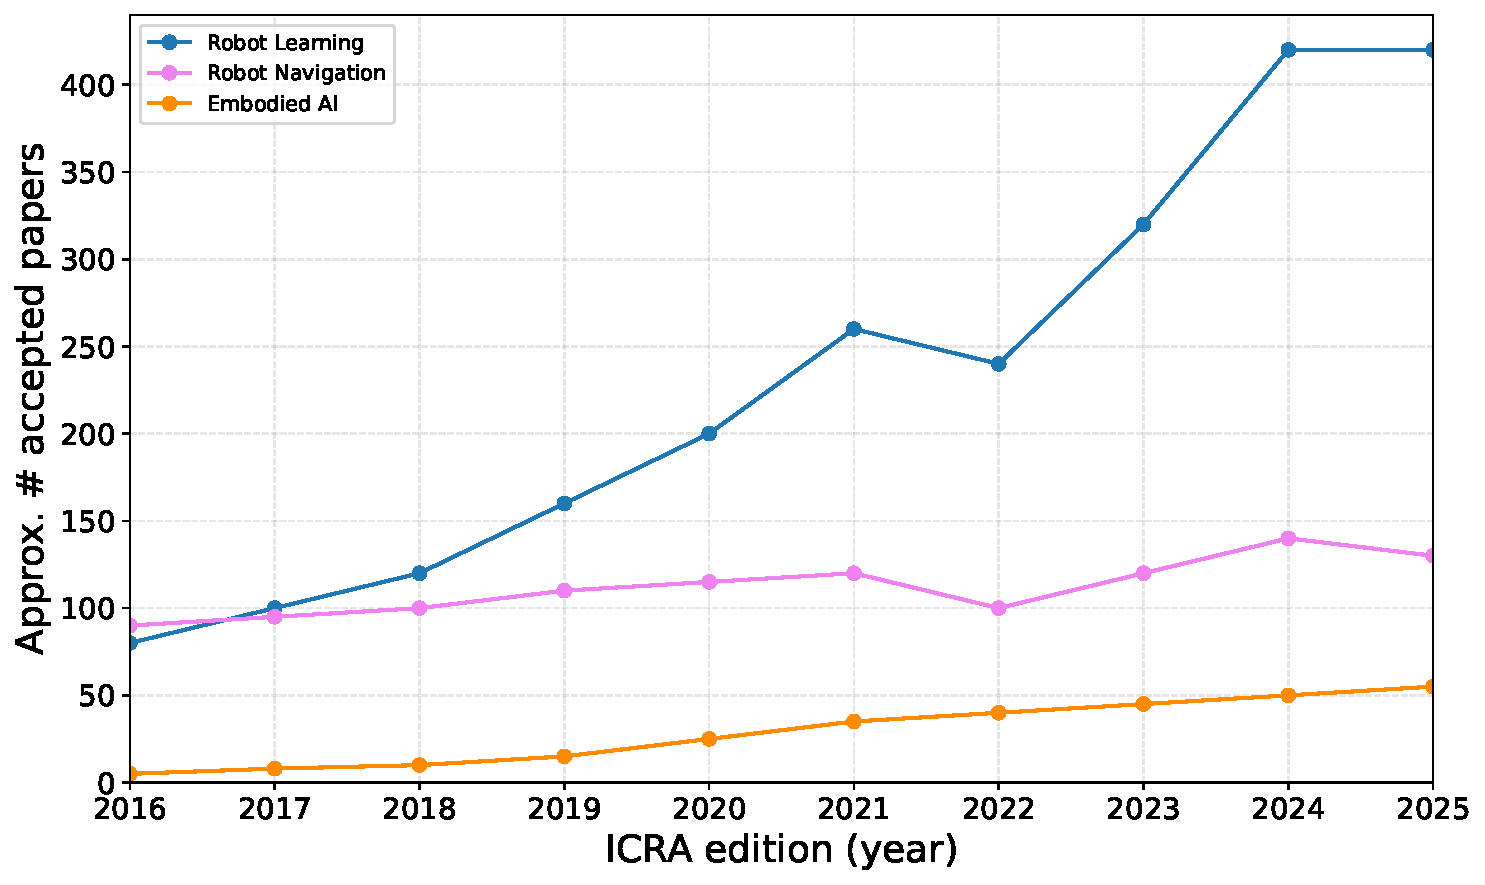
\includegraphics[width=\textwidth]{figures/introduction/icra_papers}
    \caption{\textbf{Robot learning, navigation, and embodied AI accepted papers on IEEE International Conference on Robotics and Automation (ICRA) over the last ten years}. The number of accepted papers is calculated by rule-based grep over the abstracts of the accepted papers in the ICRA proceedings. They show how typical topics in robotics that study \acrshort{vsn} have been gaining popularity over the years.}
    \label{fig:icra_papers}
\end{figure}

Beyond the research project that motivates this thesis, the ultimate goal of this thesis is to provide a comprehensive study of \acrshort{vsn} and \acrshort{rl} algorithms that can be helpful for many applications.
Some of these applications, but not all, include:
\begin{itemize}
    \item \textbf{Assistive robots}: Robots that can help people with functional diversity to navigate in their environment and perform daily tasks.
    These robots need to be able to develop enough intelligent behaviors to understand the environment and the people in it, and to adapt to their needs.
    \item \textbf{Hazardous environments}: Robots that can navigate in environments that are dangerous for humans, such as disaster areas or nuclear plants.
    They can circumvent obstacles, find victims, or even perform tasks that are too dangerous for humans.
    This is a powerful application of \acrshort{vsn} that can save lives and reduce risks for humans.
    \item \textbf{Vertical-farm inspection robots}: Robots that can navigate densely packed hydroponic racks, visually distinguish crop maturity or disease markers, and localize specific trays for targeted harvesting or treatment.
    \item \textbf{Planetary or subterranean exploration rovers:} build semantic maps of unseen caves, lava tubes, or Martian terrain, finding scientific targets while avoiding hazardous slopes without GPS\@.
    \item \textbf{Immersive VR/AR game characters:} NPCs use the same visual scene the player sees (no cheat-sheet nav meshes) so they naturally avoid furniture, peek around corners, and respond to spoken commands (“guard the green door”).
\end{itemize}

\section{Contributions of the Thesis}\label{sec:contributions-of-the-thesis}

The main contributions of this thesis are summarized as follows:
\begin{itemize}
    \item A comprehensive study of the literature of the \acrshort{vsn} setting and a thorough study of the \acrshort{rl} algorithms that can be applied to real-world scenarios.
    This includes a review of the state-of-the-art methods, their limitations, and the challenges that need to be addressed.
    Thanks to this, the ready can understand the current state of the art in \acrshort{vsn} and \acrshort{rl} and contextualize the main goals of this document.
    \item A clear definition of the \acrshort{vsn} problem and a set of benchmarks that can be used to evaluate the performance of \acrshort{vsn} algorithms in simulated environments.
    It also includes a set of metrics that can be used to evaluate the performance of different techniques such as $\epsilon$-greedy exploration or different reward functions.
    \item A comprehensive study of the different \acrshort{vsn} algorihtms in real-world scenarios.
    This includes a definition of an experimental setup that can be used to evaluate the performance of different models in real-world environments.
    On top of that, this also includes the release of a novel \acrfull{ROS} package called ROS4VSN that provides a set of tools and utilities to facilitate the development of \acrshort{vsn} algorithms in real-world scenarios.
    \item A novel approach to \acrshort{rl} that combines the advantages of Offline Reinforcement Learning~\cite{levine2020} with DD-PPO~\cite{Wijmans2019DDPPOLN} to train \acrshort{vsn} agents without the need to query any environment, just by using offline data.
    \item A novel approach to imitation learning via meta-learning~\cite{finnOneShotVisualImitation2017} that allows agents to learn from a few demonstrations and adapt to new environments.
\end{itemize}

\section{Thesis Structure}\label{sec:thesis-structure}

The structure of this thesis is as follows:

\begin{itemize}
    \item \textbf{Chapter~\ref{ch:related-work}}: This chapter provides a comprehensive review of the literature on \acrshort{vsn}, \acrshort{rl} sparsity and exploration methods, Offline\acrshort{rl}, and meta-imitation learning.
    This chapter will provide the reader with a clear context of the methods and techniques discussed in this thesis, and how they relate to the state of the art.
    \item \textbf{Chapter~\ref{ch:understanding-robotic-visual-semantic-navigation}}: This chapter sets a clear definition of the \acrshort{vsn} problem, and provides a set of benchmarks that can be used to evaluate the performance of \acrshort{vsn} algorithms in simulated environments.
    \item \textbf{Chapter~\ref{ch:ros4vsn:-enable-real-world-robotic-visual-semantic-navigation}}: This chapter presents ROS4VSN, a novel \acrshort{ROS} package that provides a set of tools and utilities to facilitate the development of \acrshort{vsn} algorithms in real-world scenarios.
    It also includes a comprehensive study of the different \acrshort{vsn} algorithms in real-world scenarios, and a definition of an experimental setup that can be used to evaluate the performance of different models in real-world environments.
    \item \textbf{Chapter~\ref{ch:beyond-rl}}: This chapter presents two novel approaches to \acrshort{rl} for navigation.
    In section~\ref{sec:offline_rl4rvsn} the advantages of Offline Reinforcement Learning are combined with DD-PPO to train \acrshort{vsn} agents without the need to query any environment, just by using offline data.
    In section~\ref{sec:mil-for-real-world-navigation} a novel approach to imitation learning via meta-learning is presented, which allows agents to learn from a few demonstrations and adapt to new environments.
    \item \textbf{Chapter~\ref{ch:conclusions}:} This chapter summarizes the main contributions of the thesis, discusses the limitations and future work, and concludes the thesis.
\end{itemize}

\chapter{Related Work}\label{ch:related-work}

\textbf{Visual Semantic Navigation.} We can identify in the literature the following groups of works for the \acrshort{vsn} problem, depending on the learning paradigm.
In the first group, there are those works that focus on the task of navigating to an object in realistic indoor environments, \eg~\cite{zhu2017, wijmans2020, chang2020, khandelwal2022}, using simulators and an agent based on CNNs as visual encoders and RNNs as the actor-critic head, following a RL paradigm.
The second group consists of the works that address the \acrshort{vsn} problem using imitation learning~\cite{wu2020a, ramrakhya2022} to build navigation policies from expert demonstrations.
Finally, in the third set we have the approaches using meta-learning techniques in order to be able to quickly adapt to new environments~\cite{wang2017, wortsman2019, zhang2022}.

Our work belongs to the first group.
In fact, our proposal is a simplification of the approach in~\cite{khandelwal2022}, where we build a model based on a CLIP feature extractor and two LSTMs encoders for the agent state, introducing also reward shaping~\cite{wijmans2020} and $\epsilon\text{-}greedy$~\cite{mnih2013}.

\textbf{Sparsity and exploration methods.} To address the sparse reward and exploration problems, different approaches have been proposed.
Auxiliary tasks~\cite{jaderberg2016, ye2021} help the agent to explore the environment and gather extrinsic reward by maximizing pseudo-reward functions.
Curiosity-driven exploration~\cite{pathak2017} leverages on the error of the agent's ability to predict the next state to introduce a new intrinsic reward that enables the agent to explore the environment.
When dealing with procedurally-generated environments, a curriculum learning mechanism can be incorporated so the episodes are ordered by an exploration score~\cite{zha2020b}, and then the agent imitates the best ones.
We also use procedurally-generated environments, but we rely on a RL approach combined with reward shaping~\cite{ng1999, jestel2021} and $\epsilon\text{-}greedy$~\cite{mnih2013} techniques to learn to navigate in them.


\textbf{Visual Semantic Navigation}.
To navigate in unfamiliar environments, traditional methods use depth sensors~\cite{newcombe2011, thrun2001} and RGB cameras~\cite{jones2011, sattler2018} to build geometric maps and simultaneously determine the robot's position in relation to the map.
This is known as Simultaneous Localization and Mapping (SLAM)~\cite{Kazerouni2022, campos2021, labbe2022}).
Typically, these SLAM models use heuristic algorithms to create graph-based representations of the environment, allowing the robot to visit the different nodes of the graph when navigating to specific points.
Semantic SLAM (\eg~\cite{zhang2018, rosinol2020, jin2023}) expands upon SLAM by integrating semantic data from the environment, allowing the robot to identify and store objects in memory.

A recent approach, made possible by advances in machine learning and computer vision, involves designing navigation policies that directly train deep neural networks to learn semantic information from visual observations in an end-to-end fashion (\eg~\cite{ramrakhya2022,yadav2022, gutierrez2019, khandelwal2022, chaplot2020,chang2020}).
This approach is termed \textit{visual semantic navigation} (\acrshort{vsn}).
These models often rely on the use of CNNs as visual encoders followed by RNNs; that are in charge of predicting an action distribution directly from raw input observations.
The neural networks are trained using imitation learning (IL) or reinforcement learning (RL) approaches.

When IL is applied to the visual navigation problem, navigation policies are learnt from expert demonstrations (\eg~\cite{ramrakhya2022,yadav2022}).
It can also be used combined with an RL fine-tuning phase to achieve better performance~\cite{ramrakhya2023}.

Other works focus on the use of an end-to-end RL approach to solve \objnav navigation~\cite{zhu2017, gutierrez2019, wijmans2020, khandelwal2022, Liu2022, Yadav2023OVRLV2AS, Xu2024DeepRL, YokoyamaHM3DOVONAD}.
Some authors have proposed combining the RL training with different strategies, like auxiliary tasks~\cite{ye2021}, improved visual representations via object relation graphs~\cite{yang2018}, semantic segmentations~\cite{Mousavian2018} or combining audio feedback with the visual inputs~\cite{Wang2023, Kondoh2023MultigoalAN}.

Modular-learning based approaches~\cite{chaplot2020, chang2020, skillfusion, Li2023RDDRLAR, zhou2022improving, Cai2024DGMemLV, Kang2024HSPNavHS, Wang2023ProbableOL, Wasserman2023ExploitationGuidedEF, Yokoyama2023VLFMVF} decompose the navigation process in separate modules that execute different tasks.
It is common for these methods to be composed of a high-level semantic exploration module trained by RL that indicates the agent subgoals that have to be reached by a low-level navigation policy.
Modular learning can be also combined with offline RL~\cite{shah2022} techniques to leverage navigation behaviors from fixed datasets, without any additional online data collection or fine-tuning.

Finally, there are different approaches that try to tackle the problem of rapidly adapting to unseen environments in visual navigation via meta-learning~\cite{wortsman2019, luo2021, zhang2022}.
These methods are trained on a variety of different environments (usually designated as tasks) and are able to generalize to unseen environments by learning a policy that can be quickly adapted to new environments.
And the recent progress in large language models (LLMs) has led to the possibility of using them to solve the visual navigation problem~\cite{Huang2023, Zhou2023} as well.
In this case, the LLMs are used as a reasoning module in charge of understanding the semantic information present on the environment.
They then share this information with different modules in charge of navigating to the specified goal.

Our goal in this work is not to develope \acrshort{vsn} approaches, but to integrate various state-of-the-art \acrshort{vsn} models into multiple real-world robots by using our novel ROS4\acrshort{vsn} library.
Technically, we have chosen to integrate the PIRLNav~\cite{ramrakhya2023} and VLV~\cite{chang2020} models into two different robots.
These integrations required several technical adaptations, particularly in the areas of sensor data integration and navigation planning.
Overall, we are able to show how ROS4\acrshort{vsn} allows easily testing and comparing different \acrshort{vsn} methods in the real world.
To the best of our knowledge, our work is the first to develop a model agnostic ROS package for visual semantic navigation, where multiple models can be integrated.

\textbf{Simulation-to-reality transfer in robotic navigation}.
Deploying a model trained in simulation to a real robot is a challenging task.
Due to logistical constraints, training a model in the real world —especially with RL techniques— is often impractical, prompting the use of alternative methods to address this challenge
For example, \cite{kim2022} propose a monocular vision-based time-to-collision estimation for small drones by domain adaptation of simulated images.
Their method converts simulated images into real-like synthetic images using a sim-to-real method.
This is done with the aim of minimizing efforts and time invested in the collection of training datasets within real-world scenarios, while simultaneously maximizing the advantages inherent in simulated environments.

Overall, it is necessary to develop methods that allow to efficiently transfer the knowledge learnt in simulation to the real world~\cite{kadian2020}.
Different approaches have been proposed to solve this problem.
For instance, CAD2RL~\cite{sadeghiCAD2RLRealSingleImage2017} system achieved remarkable success in training a collision avoidance policy entirely within a simulated environment.
This breakthrough was subsequently tested on real aerial drones, with promising results.
By focusing on simulation refinement~\cite{Son2020}, the accuracy of simulations can be improved by exploiting the disparities between simulated and real-world observations.
In the field of locomotion, training legged robotic systems in a simulated environment and subsequently transferring the acquired policies to real-world applications~\cite{Hwangbo_2019, agarwal2022} has always been a challenging task.

For the problem of \acrshort{vsn}, we have the studiy by \cite{gervet2022} that shows how their approaches perform in real-world settings.
However, we would like to highlight the novel contributions that our work offers.
First, while~\cite{gervet2022} focuses mainly on the comparison of their navigation methods, we here, along with a similar study, release to the research community the modular ROS4\acrshort{vsn} software architecture.
Our main goal is to facilitate the prototyping of new \acrshort{vsn} solutions on real robots.
So, we offer a ROS-compatible software architecture, model agnostic, that allows a simple integration of different \acrshort{vsn} approaches in ROS robots.
In this way, future \acrshort{vsn} solutions will be able to be tested on real robots in a convenient and straightforward manner.
Second, we include in our study more recent \acrshort{vsn} solutions than the ones reported in~\cite{gervet2022}, as the PIRLNav model~\cite{ramrakhya2023}, which defines the state-of-the-art for the \objnav problem.
Third, we also provide, for the first time, a detailed analysis on how a model directly trained with real videos, such as the VLV~\cite{chang2020}, performs in real robots.
This allows us to compare, as in~\cite{gervet2022}, how a modular-learning model (\ie VLV~\cite{chang2020}), compares with a typical end-to-end learning approach (\ie PIRLNav).
Interestingly, our study also concludes, like in~\cite{gervet2022}, that modular-learning approaches perform better in the real world.
Fourth, in our study, we employed two different robotic platforms: one commercially available and widely used by various laboratories, and another custom-built.
This demonstrates the versatility of the proposed solution, showing that it can be integrated into different robots.
And finally, in our work, we propose an experimental evaluation specifically designed for testing in the real world, which can be employed in future research studies.
Overall, we hope that our ROS-based library will help to further advance the field of visual semantic navigation in real robots.


\section{RL For Navigation}\label{sec:navigation}

\subsection{Problem Formulation}\label{subsec:problem-formulation}

We address the VSN problem by using Reinforcement Learning (RL).
Thus, navigation can be described as a partially observable Markov decision process (POMDP), in which the agent, \ie, a robot, navigates through an environment and tries to reach a determined object.
This problem is known in the literature as the ObjectNav task~\cite{batra2020}.

Formally, given an initial observation distribution $p_0$, for the step $t$ the agent receives an observation $o_t \sim p_0(o)$ based on state $s_t$, which in our case is just an RGB image of what the robot observes.
The agent takes action $a_t$, obtains reward $r_t$ from the environment and receives a new observation $o_{t+1} = \mathcal{T} (o_{t+1}|o_t, a_t)$, where $\mathcal{T}$ is the transition function.
An episode is a sequence of $\left(o_t, a_t, r_t\right)$ tuples that form a trajectory.
The episode ends when the agent reaches the goal or the maximum number of steps ($H$).
An episode is considered a success if the agent reaches the goal within the step horizon $H$.

The goal is to find an optimal policy $\pi^*$ that maximizes the cumulative reward over an episode.
This policy maps observations to a probability distribution over actions that is specified as follows,
\begin{equation}
    \label{eq:op_policy}
    \pi^*=\argmax\limits_\pi\mathbb{E}_{\mathcal{T}\sim\pi}[R_H],
\end{equation}
where $R_H=\sum_{t=1}^H \gamma^{t-1}r_t$ is the return, \ie the cumulative reward over an episode, and $\gamma$ is a discount factor.
In navigation tasks, neural networks with parameters $\theta$ are often used to parameterize the policy $\pi_\theta$.

\subsection{Visual Semantic Navigation}\label{subsec:visual-semantic-navigation}

Learning to navigate in a given environment is a challenging task.
First, the reward signal coming from the environment is usually sparse~\cite{sutton2018, pathak2017}.
These sparse rewards lead to a quite difficult training process.
%Second, the agent has to balance an exploration of the environment to obtain experience and the exploitation of the previous experience in order to obtain successful episodes~\cite{sutton2018, mnih2013}.
Second, we need to find a balance between the exploration and exploitation of the environment to achieve successful experiences that drive the agent's learning process~\cite{sutton2018, mnih2013}.
Finally, the agent architecture has a direct impact on how it learns.
State-of-the-art approaches use a feature extractor followed by recurrent units to process temporal information coming from the images.
%For navigation tasks, a common agent architecture consists of a CNN feature extractor and an RNN that outputs the action distribution.

\textbf{Sparse rewards and long horizon.}
%In visual navigation, sparse rewards are a common issue due to the nature of the task, \ie reaching a specific target in an environment.
Sparse rewards are a common issue due to the nature of the navigation tasks, \ie reaching a specific target in an environment.
The most straightforward way to define a reward in navigation problems is to let the environment provide a fixed amount when the agent reaches the goal.
This means the agent has to face an environment in which:
1) in the best case, most of the reward signal is zero except for the step in which the agent reaches the goal and obtains a certain amount of reward;
and 2) if the agent does not reach the target it does not receive any reward.
This situation worsens with large temporal horizons, because the more steps, the higher the sparsity of the reward is.

To mitigate the sparse reward problem, we use a technique called reward shaping.
It consists in modifying the original reward signal via incorporating domain knowledge.
For navigation, we leverage on the \textit{distance reward}~\cite{wijmans2020}, defined as:
\begin{equation}
    \label{eq:rew_shaping}
    r_t = -d(s_t, target) + d(s_{t+1}, target) - r_s + r_T,
\end{equation}
where $d(s_t, target)$ computes the geodesic distance between agent's position at state $s_t$ and $target$'s position.
$r_T$ is the \textit{terminal reward}, a fixed amount given only when the agent reaches the target and $r_s=0.01$ is the \textit{slack reward}, also a fixed amount that penalizes each step.
The goal of the \textit{distance reward} function is to give a constant reward signal to the agent that increases as the agent approaches the target.
In section~\ref{subsec:miniworld-maze-results} we compare the \textit{distance reward} against what is usually referred to as the \textit{navigation reward}, which consists only of the slack reward and the terminal reward $r_t = -r_s + r_T$.

\textbf{Exploration vs. Exploitation.}
%As we have mentioned, in a navigation problem, our agent must explore the environment in order to find the trajectories that return the maximum amount of reward without surpassing the temporal horizon of $H$ steps.
%This exploration has to be balanced with respect to the exploitation process, in which the agent uses the previous knowledge to actively select the best actions to obtain the shortest successful episodes.
As we have mentioned, the exploration process has to be managed to encourage the agent to choose actions that it would not otherwise select.
To address this issue, we leverage the technique known as $\epsilon\text{-}greedy$~\cite{mnih2013}.
This solution \emph{controls} the action that is being selected by the agent, usually during the learning process.
Given an $\epsilon \in [0, 1]$, an action $a_t$ is selected as
\begin{equation}
    \label{eq:eps-greedy}
    a_t = \begin{cases}
              \argmax\pi_\theta & \mbox{with probability 1-$\epsilon$,}     \\
              rand(a) \in \mathcal{A} & \mbox{with probability $\epsilon$,} \\
    \end{cases}
\end{equation}
where $\mathcal{A}$ defines the action space.
Typically, $\epsilon$ starts at $1$ and it decays with the iterations.
In the beginning of the learning process, \ie when $\epsilon$ is high, random actions are sampled more often, encouraging the agent to explore the environment.
As the training process advances, lower $\epsilon$ values permit the agent to exploit the model knowledge to select the best action.
This introduces a balance between exploration and exploitation.

\textbf{Agent architecture.} We encode the agent as a parameterized model consisting in a CLIP~\cite{khandelwal2022} visual encoder connected to two actor-critic LSTMs that output a discrete distribution over the action space and the value, respectively.
A diagram of the implemented agent can be found in figure~\ref{fig:network_clip_diagram}.
To train the models, we use Proximal Policy Optimization (PPO)~\cite{schulman2017}, an on-policy RL algorithm.

\begin{figure}[t]
    \centering
    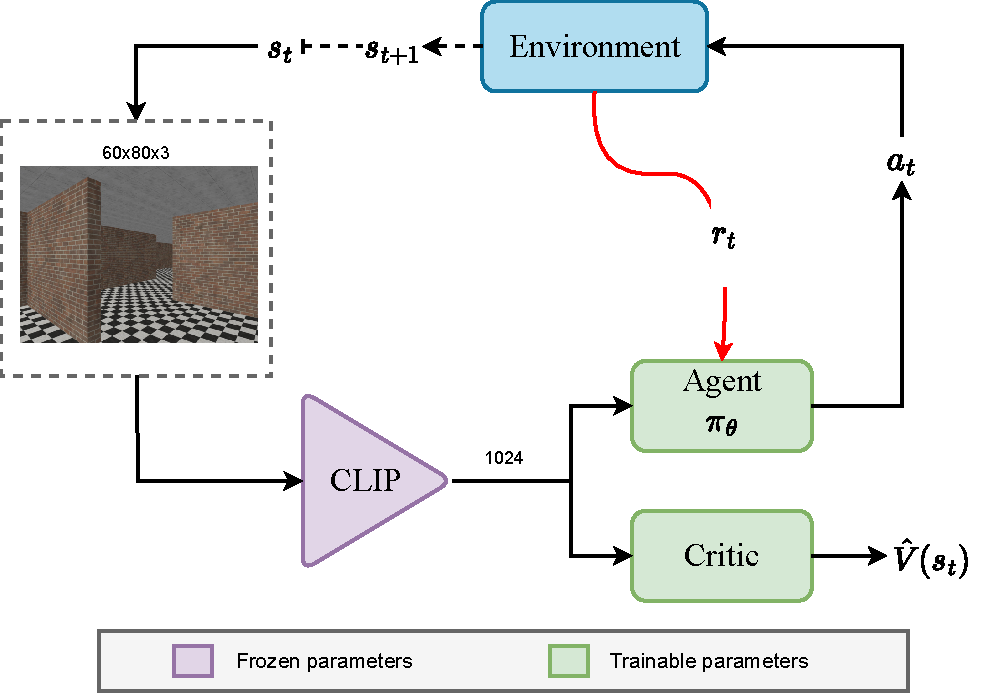
\includegraphics[width=0.8\linewidth]{graphics/network_clip_diagram}
    \caption{\textbf{Model diagram}. This figure contains a high level representation of the model used: a visual encoder followed by an actor-critic module encoded by LSTMs. The visual encoder is frozen and we only train the actor-critic module.}
    \label{fig:network_clip_diagram}
\end{figure}


\section{Experiments and Results}\label{sec:experiments}

Is an offline RL algorithm able to learn navigation policies effectively?
To answer this question, we have trained our DD-IQL model using the expert demonstrations on five different experimental setups.
These setups have been designed with an incremental difficulty.
The first three are evaluated on the same environments in which the agents were trained, while the last two are evaluated on different environments.
The details of the setups are depicted on figure~\ref{fig:setups}.

We compare our results with the current state-of-the-art model PirlNav~\cite{ramrakhya2023}.
This model is based on a two-phase training schedule.
The first phase is a supervised learning phase, where the model is trained using behavior cloning on the expert demonstrations.
The second phase is a reinforcement learning phase, where the model is fine-tuned using DD-PPO~algorithm~\cite{wijmans2020}.
For a fair comparison, we train the PirlNav agent using only the behavior cloning phase on the same setups as our OffNav model.

Results are shown on table~\ref{tab:success}.
It can be seen that both methods obtain similar performance on setups 1 to 3.
Offnav method outperforms PirlNav on setup 2, while PirlNav outperforms OffNav on setup 3, and both of them obtain $100\%$ SR on setup 1.
When evaluated on setup 4, PirlNav outperforms OffNav by $2.27\%$ absolute points.
However, on setup 5, the most challenging one, OffNav outperforms PirlNav by $8.69\%$ absolute points.


\begin{table}
    \centering
    \begin{tabular}{c|ccc}
        \toprule
        \textit{Experimental Setup} & \textit{OffNav}  & \textit{PirlNav} \\
        \midrule
        \textsc{Setup 1}            & 100\%          & 100\%   \\
        \textsc{Setup 2}            & \textbf{79.31\%} & 72.50\%          \\
        \textsc{Setup 3}            & 75.78\%          & \textbf{77.63\%} \\
        \textsc{Setup 4}            & 25.00\%          & \textbf{27.27\%} \\
        \textsc{Setup 5}            & \textbf{34.78\%} & 26.09\%          \\
        \bottomrule
    \end{tabular}
    \caption{Success Rate for OffNav and PirlNav methods on the five experimental setups.}
    \label{tab:success}
\end{table}

\begin{figure}
    \centering
    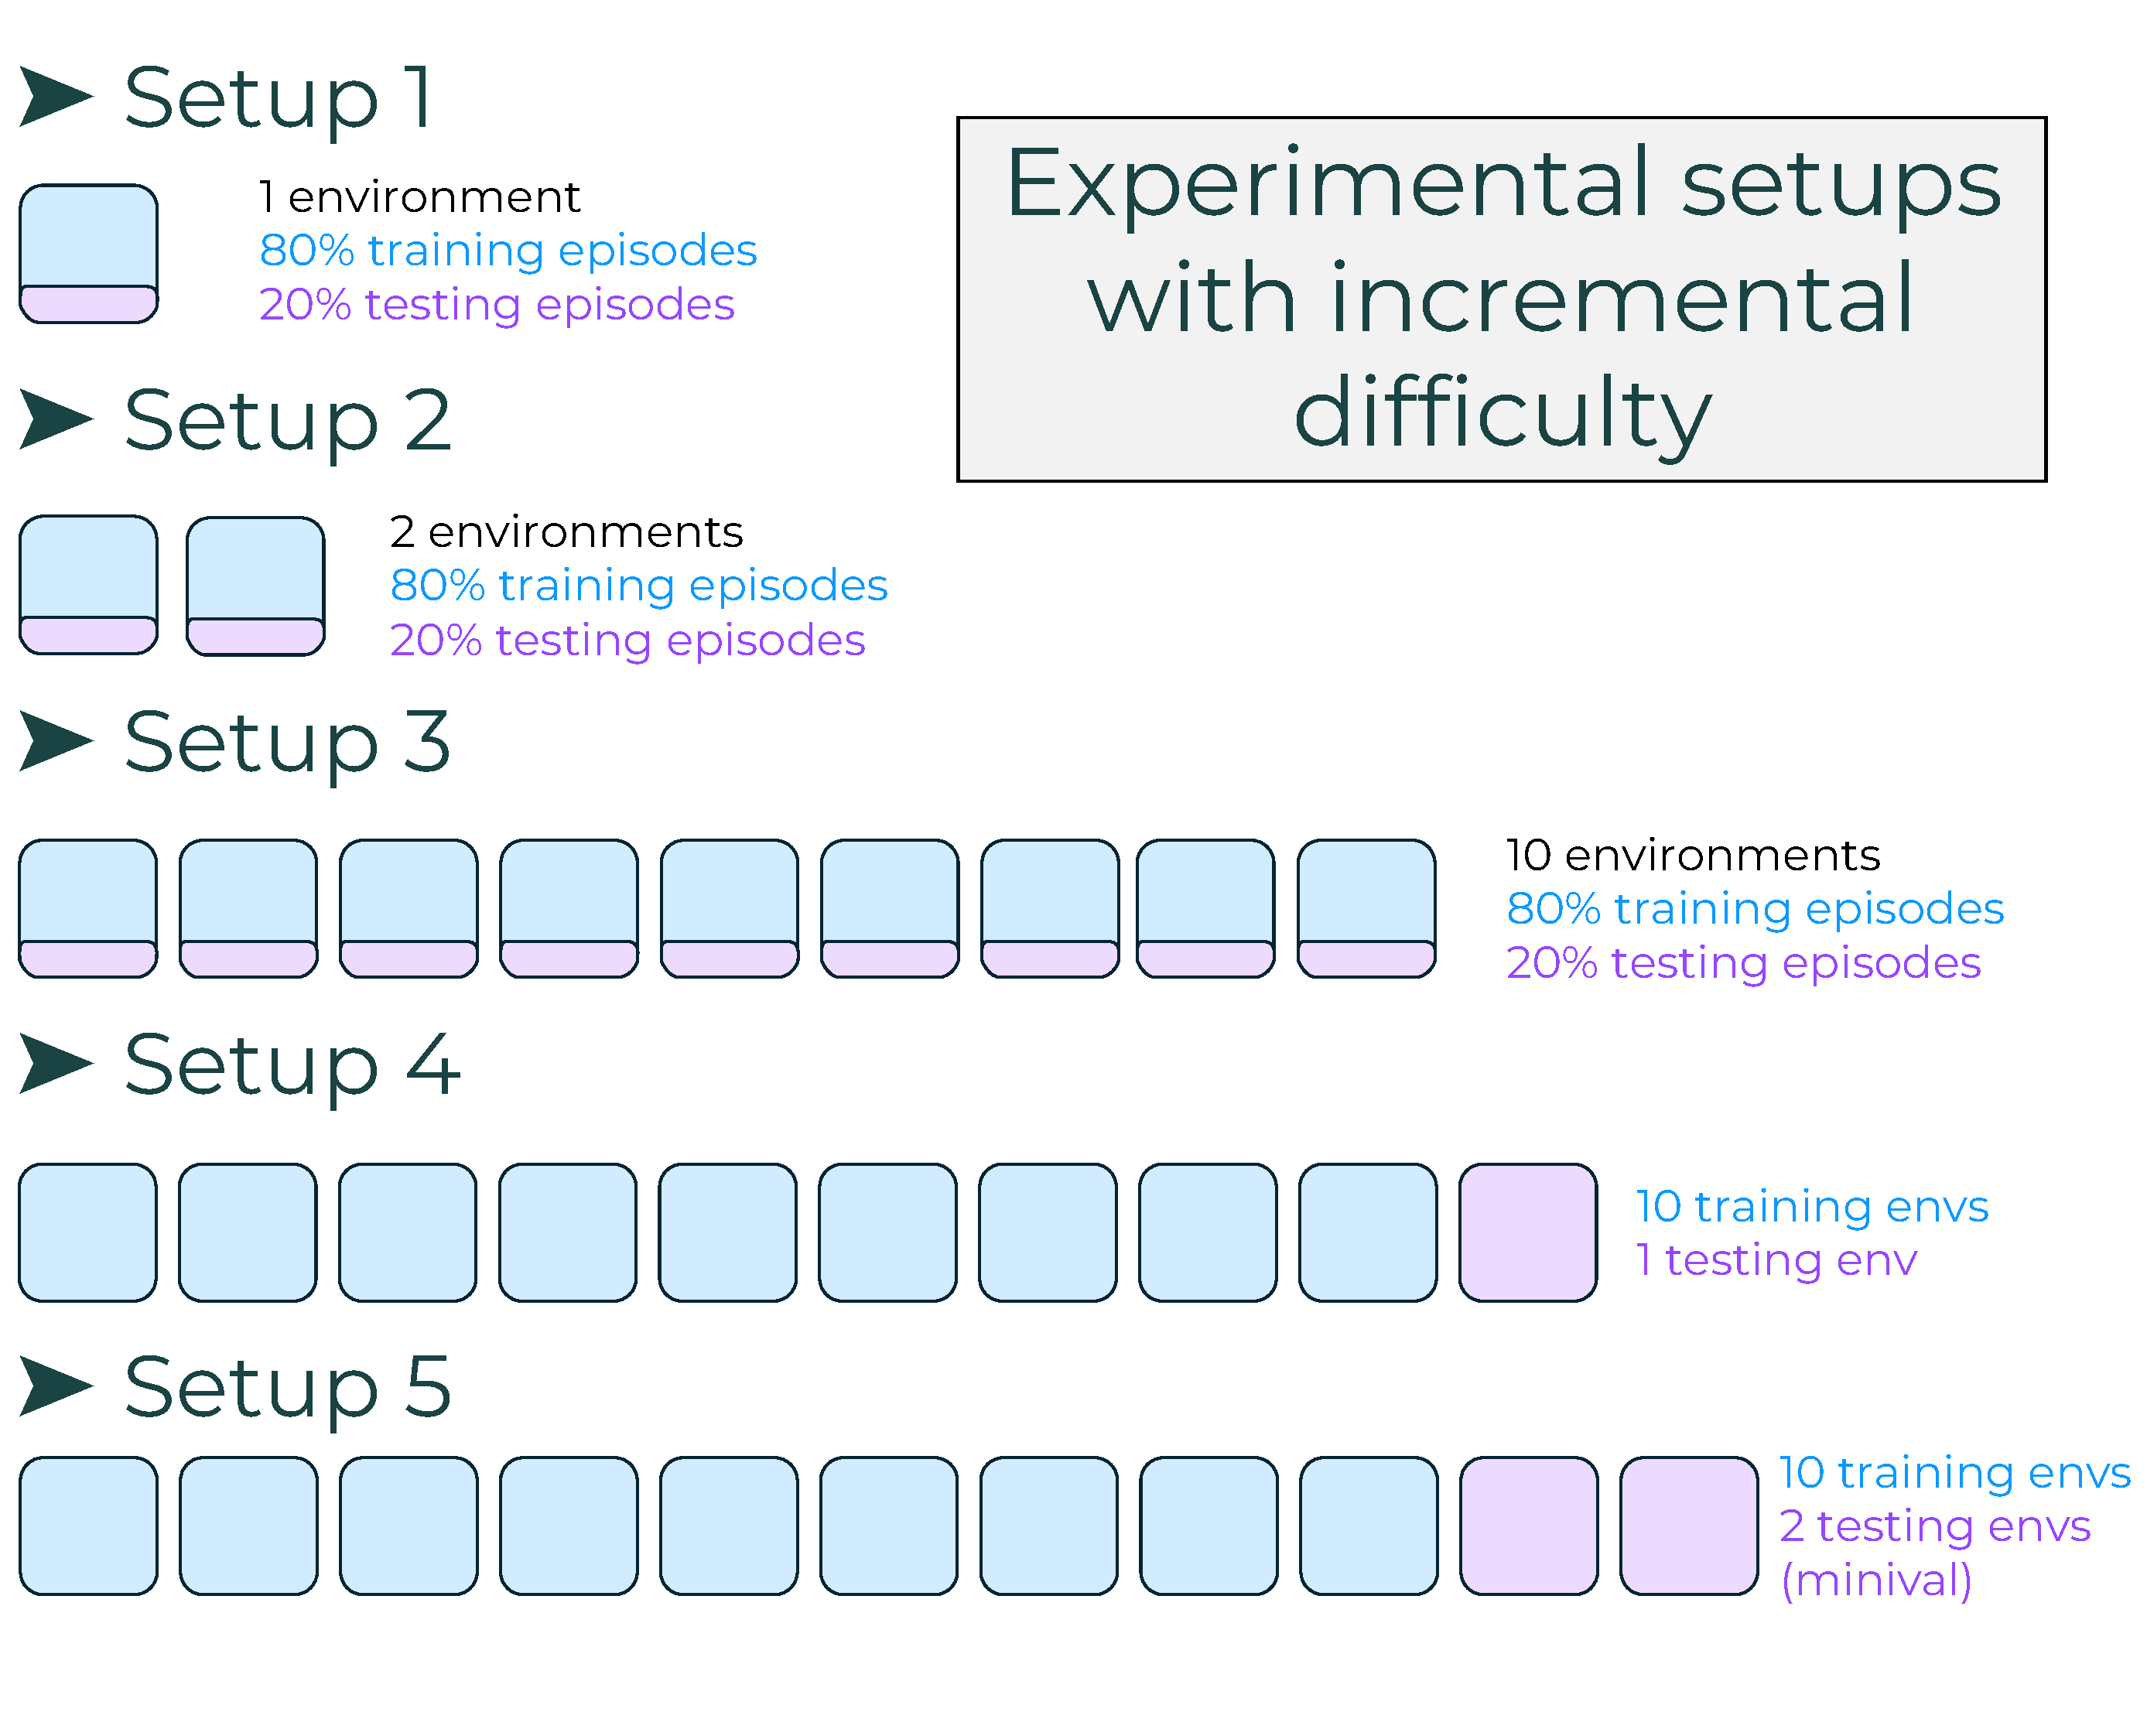
\includegraphics[width=\linewidth]{figures/experimental_setups}
    \caption{Five experimental setups designed with an incremental difficulty.}
    \label{fig:setups}
\end{figure}






\chapter{Conclusions}\label{ch:conclusions}

\lettrine{\textcolor{accent_color}{T}}{his} thesis has focused on the exploration of robotic visual navigation, specifically in the context of visual semantic navigation, and how it can be improved through the use of reinforcement learning methodologies.
The main objective has been to develop a new ROS~\cite{ros} framework that allows the integration of different algorithms and environments, as well as to explore new approaches to offline reinforcement learning and meta imitation learning for robotic visual navigation.
Concretely, the thesis has focused into studying and solving the \acrshort{objnav} problem in the real world, which consists of navigating to a specific object instance in an determined environment using visual information.
This is a challenging task since it involves a combination of several abilities, such as visual perception, semantic understanding, and navigation in complex environments.

This problem has been heavily dependent on the use of simulated environments for training and evaluation, which has limited the applicability of the developed algorithms in real-world scenarios.
However, it is not until recent years that the use of real-world data for evaluation has become more common, allowing for a better understanding of the limitations and challenges of the developed algorithms in real scenarios.
In this scenario, the thesis focuses on studying the limitations of the current approaches to robotic visual navigation in the real world, and how they can be improved through the use of new methodologies and frameworks.

This chapter summarizes the main contributions derived from the research carried on while the development of this thesis.
It also tackles the discussion and limitations of the proposed approaches, as well as the future research lines that can be explored to further improve the state of the art in robotic visual navigation.
Finally, it summarizes the scientific contributions derived from this thesis, both directly related to the main topic and side contributions that have been developed in parallel.

\section{Contributions}\label{sec:contributions}

Broadly, the thesis has contributed to the topics of \acrfull{vsn} and different algorithms for it in the context of robotic visual navigation, and how they can be improved through the use of new methodologies and frameworks.

\subsection{Contributions to the study of Visual Semantic Navigation}\label{subsec:contributions-to-visual-semantic-navigation}

The \acrshort{vsn} problem has been a challenging task in the field of robotics, and almost all the proposed solutions laid on the use of reinforcement learning methodologies.
The problem with reinforcement learning in the machine learning field is that it is a less industrialized field than others, like supervised learning or generative models.
This has lead to a diverse use of several \acrshort{RL} libraries and frameworks, which has made it difficult to compare the results of different approaches and to reproduce the results of previous works.
Also, the use of simulated environments for training and evaluation has limited the applicability of the developed algorithms in real-world scenarios.

To address these issues, this thesis has proposed two solutions: a thorough study for evaluation protocols in \acrshort{VSN} and the development of a new framework for robotic visual navigation that allows the integration of different algorithms in real environments.
The following list details the main contributions to the field of \acrshort{vsn} that have been developed during the thesis:

\begin{itemize}
    \item An intensive study of the current state of the art in \acrshort{vsn} and its limitations, which has allowed to identify the main challenges and opportunities for improvement in this field.
    The review of the literature helped to identify tantos important aspects:
        \begin{enumerate}
            \item There is a lack of standarized frameworks and protocols for training and evaluating \acrshort{vsn} algorithms, which has made it difficult to compare the results of different approaches and to reproduce the results of previous works.
            \item Almost all the proposed solutions to \acrshort{vsn} are based on simulation, and while this is a common practice in the field of robotics, it does not allow for a realistic measurement of the performance of the algorithms in the real world.
            \item Although plenty of methods have been proposed to solve the \acrshort{vsn} problem, and even some of them have been tested in real robots, there is a lack of methods developed specifically for real-world scenarios, and how to quickly adapt them to new environments.
        \end{enumerate}
    \item A new \acrshort{vsn} model that leverages CLIP~\cite{radford2021} encoders to process the visual information followed by an RNN module to output the navigation actions.
    \item An evaluation of different \acrshort{rl} techniques to deal with the sample inefficiency~\cite{Yarats2019ImprovingSE} problem of online reinforcement learning: \textit{reward shaping} and $\epsilon-greedy$~\cite{mnih2013}.
    \item The design of a new thorough experimental evaluation protocol for \acrshort{vsn} in simulation implemented via pyRIL~\cite{pyRIL} for two navigation environments: Miniworld-Maze~\cite{gym_miniworld} and Habitat~\cite{szot2021}.
    \item The release of a new \acrshort{ros} framework for deployment of \acrshort{vsn} algorithms in real robots.
    It allows the integration of different algorithms and environments and provides a standardized way to use them.
    \item The first time that two state-of-the-art \acrshort{vsn} algorithms (PIRLNav~\cite{ramrakhya2023} and VLV~\cite{chang2020}) have been evaluated in real robots, which has allowed to identify the main challenges and limitations of the current approaches in real-world scenarios.
    \item A new experimental evaluation for \acrshort{vsn} algorithms in the real world using the proposed \acrshort{ros} framework, which has allowed to measure the performance of the algorithms in real-world scenarios and to identify the main challenges and limitations of the current approaches.
\end{itemize}

\subsection{Contributions to the development of new algorithms for Visual Semantic Navigation}\label{subsec:contributions-to-new-algorithms-for-visual-semantic-navigation}

The thesis has also contributed to the development of new algorithms for \acrshort{vsn} that can be used in real-world scenarios.
While these algorithms resemble the same problem formulation used for \acrshort{rl}, they are not based on classical \acrshort{rl} methodologies but rather on offline reinforcement learning and meta-imitation learning.
These approaches aim to go \textit{beyond} the current \acrshort{rl} methodologies and try to provide a foundation for future research in algorithms that are meant to overcome the limitations of \acrshort{rl} in the real world.

Specifically, the following contributions have been made:

\begin{itemize}
    \item A new simplified experimental evaluation protocol for HM3D~\cite{ramakrishnan2021} dataset, based on five different setups that increase the complexity of the navigation task.
    This allows for faster training and evaluation of algorithms.
    \item A new approach to \acrshort{vsn} based on offline reinforcement learning called \textbf{Off}line Visual Semantic \textbf{Nav}igation (OffNav).
    This approach allows training \acrshort{vsn} algorithms using offline data, which can be collected in real-world or simulated scenarios.
    This algorithm is based on the Implicit Q-Learning (IQL)~\cite{kostrikov2022offline} algorithm, but adapted to decentralized distributed training and evaluation.
    The model is able to generalize to unseen environments and in the most challenging setup it outperforms the state-of-the-art PIRLNav~\cite{ramrakhya2023} algorithm.
    \item A novel model for \acrshort{vsn} based on meta-imitation learning called \textbf{Meta} Imitation Learning for Visual Semantic \textbf{Nav}igation (MetaNav).
    This approach allows training navigation policies using pre-recorded demonstrations in a meta-learning fashion.
    The model is an adaptation from~\cite{finnOneShotVisualImitation2017} to work in the \objnav setting.
\end{itemize}

\section{Discussion and Limitations}\label{sec:discussion-and-limitations}

As any research works, this thesis provides more questions than answers.
Besides the contributions listed in the previous sections, there are several elements that could be addressed to improve the work here done.
Although some of them represent limitations and challenges that have been identified during the development of this thesis, there are others than resemble all the possibilities unexplored.
Some of these elements are listed below:
\begin{itemize}
    \item The \acrshort{vsn} models employed alongside this thesis are always based on the same principle: a visual feature extractor (typically CNNs, but not limited to) plus RNNs to output action distributions.
    This is a good starting point and has been identified as a strong baseline for navigation models~\cite{wijmans2020}.
    However, navigation could be improved by using more recent architectures, such as transformers~\cite{Vaswani2017AttentionIA} or diffusion~\cite{pmlr-v37-sohl-dickstein15} models, which have shown to be also effective in embodied AI tasks~\cite{Shah2023ViNTAF, ren2025prior}.
    \item All the proposed algorithms and analysis performed for \acrshort{vsn} are based on the same task formulation: navigating to a specific object instance in an environment, known as \acrshort{objnav}.
    While this is still a challenging task, specially in the real world and dynamic environments, there are other tasks that could be explored.
    As expressed in chapter~\ref{ch:introduction}, if we want a robot to be able to interact with the environment as humans, it has to be able to perform more complex tasks than just navigating to a specific object instance.
    There are plenty of tasks that could be explored.
    Some of them, but not all are: vision and language navigation~\cite{Anderson2017VisionandLanguageNI}, in which and agent has to navigate to a specific location in an environment based on a natural language instruction; HAZARD navigation~\cite{Zhou2024HAZARDCE}, in which an agent has to rescue a given set of objects from disasters such as fires, floods, and winds; Open-Vocabulary Mobile Manipulation~\cite{homerobotovmm, homerobotovmmchallenge2023}, which is the problem of picking any object in any unseen environment, and placing it in a commanded location; or even more dynamic tasks such as Social Navigation~\cite{puig2024habitat}, a set of tasks that involve cooperation between multiple agents or agents and humans.
    Some of these tasks can be about navigating in an environment while avoiding moving humans, or even rearranging objects in coordination with a human agent.
    \item While this thesis proposes two new algorithms for \acrshort{vsn} based on offline reinforcement learning and meta-imitation learning in chapter~\ref{ch:beyond-rl}, these algorithms struggle to outperform the state-of-the-art algorithms in the most challenging setups.
    As pointed out in section~\ref{sec:training-problems}, both algorithms suffer from an inability to be trained in the full HM3D dataset train split.
    While further research is needed to understand the limitations of these algorithms, the experimental evidence suggests that the heavy modifications made to the original algorithms made them actually less effective than the original ones.
    \item As the algorithms from chapter~\ref{ch:beyond-rl} showed bad performance in the most challenging setups, they were not tested in real robots.
    However, tests on real robots are crucial to understand the limitations of the algorithms and how they can be improved, and they could have shown crucial insights on how to improve the algorithms.
    \item All the algorithms studied or proposed in this thesis are based on robot learning.
    All of them have at least one component trained using reinforcement learning or imitation learning.
    However, these algorithms do not represent the whole space of algorithms that can be used for \acrshort{vsn}, and in more general any robotic task.
    Moreover, these other algorithms can be used in conjunction with the proposed algorithms to improve their performance.
    Nonetheless, this thesis is focused on learning algorithms, and other methods such as planning, control, or even classical computer vision methods are out of the scope.
\end{itemize}

\section{Future Research Lines}\label{sec:future-work}

Despite much effort has been put into the development of this thesis, the ultimate goal of achieving a fully autonomous robot that can navigate and interact with the environment as humans do is still far from being achieved.
Apart from all the required research that has to be made in order to fulfill the limitations and challenges listed in the previous section, there are several research lines that can be explored to further improve the state of the art in robotic visual navigation.

First of all, despite the algorithms presented in chapter~\ref{ch:beyond-rl} are meant to bridge the gab between simulation and real-world scenarios, they have not been tested in real robots.
By leveraging on the framework ROS4VSN proposed in chapter~\ref{ch:ros4vsn:-enable-real-world-robotic-visual-semantic-navigation}, these algorithms can be easily deployed in real robots and tested in real-world.
This is the most immediate research line that can be explored, as it will reflect how these algorithms perform in real-world scenarios and how they can be improved.
Nevertheless, developing algorithms in simulation and testing them in real robots is only the first step, even if they are meant to be used in real-world scenarios.
The problem is that normal simulation time for end-to-end reinforcement learning algorithms surpasses that of a human lifetime.
However, typically, humans are able to interact with an environment as soon as they reach their first year of life.
This difference in learning time is due to the sample inefficiency of reinforcement learning algorithms, which is a well-known problem in the field.
Making algorithms that can learn from real-world data in the same time as humans (or even faster) is a challenging task, but it is crucial to achieve fully autonomous robots.

Second, in the particular case of MetaNav, proposed in section~\ref{sec:meta-imitation-learning}, there is one immediate research line that can be explored.
Instead of using meta-imitation learning via a gradient-based approach, task-inference methods~\cite{Beck_2025, rakelly2019} can be used.
These methods allow conditioning the policies to task representations, which can be meta-learned from the training tasks.
This would allow for the main components of the model to be trained in the same fashion as the original algorithm, but with the added contextual information provided by the task representations.
In the particular case of \acrshort{objnav}, these task representation could be inferred by some geometrical distribution of the object instances in the environment, such as the distance to the goal object, or even the visual features of the object.

Finally, this since thesis has focused on the \acrshort{objnav} problem, all the algorithms and approaches proposed and analyzed only use visual information to navigate in an environment.
However, there are other sources of information that can be used to improve the performance of the algorithms.
For instance, the use of audio signals~\cite{Kondoh2023MultigoalAN} can be used to improve the performance of the algorithms in real-world scenarios, as it can provide additional information about the environment and the objects in it.
Another example is the use of tactile sensors~\cite{Ota2023TactileEO}, which can provide additional information about the objects in the environment and can be used to improve the performance of the algorithms in real-world scenarios.

These are just some examples of the many research lines that can be explored to further improve the state of the art in robotic visual navigation.
Fortunately, the field of robotics is constantly evolving, and new approaches and methodologies are being developed every day.

\section{Scientific Contributions}\label{sec:final-remarks}

During the development of this thesis, there have been contributions to several topics.
Most of them are directly related to the main topic of the thesis.
However, it has also been possible to contribute to other topics that, although not directly related to the thesis, have been developed in parallel.
These have come from side projects or collaborations with other research groups and have contributed to the development of this thesis.
All of them are summarized in the following subsections.

\subsection{Contributions directly related to the thesis}\label{subsec:contributions-directly-related-to-the-thesis}

\begin{itemize}
    \item \cvpub{\textbf{Gutiérrez-Alvarez C.}, Ríos-Navarro P., Flor-Rodríguez-Rabadán R., Acevedo-Rodríguez F.J., López-Sastre R.J., \textit{Visual Semantic Navigation with Real Robots}, in Applied Intelligence, 2024.}
    \item \textbf{Gutiérrez-Alvarez C.}, Acevedo-Rodríguez F.J., López-Sastre R.J., Kanezaki A., OffNav: \textit{Offline Reinforcement Learning for Visual Semantic Navigation}, in ICRA Human-aligned Reinforcement Learning for Autonomous Agents and Robots Workshop, 2024.
    \item \textbf{Gutiérrez-Alvarez C.}, Ríos-Navarro P., Flor-Rodríguez-Rabadán R., Acevedo-Rodríguez F.J., López-Sastre R.J., \textit{Evaluation of Visual Semantic Navigation Models in Real Robots}, in IROS Late Breaking Results, 2023.
    \item \textbf{Gutiérrez-Alvarez C.}, Hernández García S, Nasri N, Cuesta-Infante Alfredo, López-Sastre RJ, \textit{Towards Clear Evaluation of Robotic Visual Semantic Navigation}, in ICARA, 2023.
    \item \textit{Participation in the project \textbf{NAVIGATOR-D} (PID2023-148310OB-I00)}, funded by the Spanish Ministry of Science and Innovation.
    \item \textit{Participation in the project \textbf{AIRPLANE} (PID2019-104323RB-C31)}, funded by the Spanish Ministry of Science and Innovation.
\end{itemize}

\subsection{Side contributions}\label{subsec:side-contributions}

\begin{itemize}
    \item Flor-Rodríguez-Rabadán R., \textbf{Gutiérrez-Álvarez C.}, Acevedo-Rodríguez F.J., Lafuente-Arroyo S., López-Sastre R.J., \textit{SEMNAV: A Semantic Segmentation-Driven Approach to Visual Semantic Navigation}, in ArXiv, 2025.
    \item Blanco-Fernández E., \textbf{Gutiérrez-Alvarez C.}, Nasri N., Maldonado-Bascón S., López-Sastre R.J., \textit{Live Video Captioning}, in Multimedia Tools and Applications, 2025.
    \item Nasri N, \textbf{Gutiérrez-Álvarez C.}, López-Sastre RJ, Lafuente-Arroyo S., Maldonado-Bascón S. \textit{Realistic Continual Learning Approach using Pre-trained Models}, in ArXiv 2024.
    \item Lafuente-Arroyo S., Maldonado-Bascón S., Delgado-Mena D., \textbf{Gutiérrez-Alvarez C.}, Acevedo-Rodríguez F.J., \textit{Multisensory Integration for Topological Indoor Localization of Mobile Robots in Complex Symmetrical Environments}, in Expert Systems with Applications, 2023.
    \item Nasri N, López-Sastre RJ, Pacheco-da-Costa S, Fernández-Munilla I, \textbf{Gutiérrez-Álvarez C.}, Pousada-García T, Acevedo-Rodríguez FJ, Maldonado-Bascón S. \textit{Assistive Robot with an AI-Based Application for the Reinforcement of Activities of Daily Living: Technical Validation with Users Affected by Neurodevelopmental Disorders}, in Applied Sciences, 2022.
\end{itemize}

% \section*{Acknowledgment}
% This research was funded by project AIRPLANE, with reference PID2019-104323RB-C31, from the Ministry of Science and Innovation of Spain.

\bibliographystyle{IEEEtran}
\bibliography{library}

\end{document}
